\documentclass[apj]{emulateapj}

%Specify packages
\usepackage{amsmath}
\usepackage[tight]{subfigure}
\usepackage[breaklinks,colorlinks,citecolor=blue]{hyperref}
\usepackage[all]{hypcap}
\usepackage[utf8]{inputenc} %force unicode in bibtex
\usepackage{enumitem}
%use for editing/highlighting
\usepackage{color,soul}
\usepackage{lipsum}
%\usepackage{lineno}

%Define new commands as needed
\newcommand{\ang}{\AA~}
\defcitealias{barnes_inference_2016-1}{Paper II}
\renewcommand{\sectionautorefname}{Section}
\renewcommand{\subsectionautorefname}{Subsection}
%\linenumbers
%Set options for list spacing
\setenumerate{noitemsep}

\begin{document}
	%Frontmatter
	\title{Inference of Heating Properties from ``Hot'' Non-flaring Plasmas in Active Region Cores I. Single Nanoflares}
	%Authors
	\author{W. T. Barnes}
	\affil{Department of Physics \& Astronomy, Rice University, Houston, TX 77251-1892}
	\email{will.t.barnes@rice.edu}
	%
	\author{P. J. Cargill}
	\affil{Space and Atmospheric Physics, The Blackett Laboratory, Imperial College, London SW7 2BW}
	\affil{School of Mathematics and Statistics, University of St. Andrews, St. Andrews, Scotland KY16 9SS}
	%
	\and
	%
	\author{S. J. Bradshaw}
	\affil{Department of Physics \& Astronomy, Rice University, Houston, TX 77251-1892}
	%Affiliations
	%Abstract
	\begin{abstract}
		\hl{Abstract will go here.}
	\end{abstract}
	%Body
	\section{Introduction}
	\label{sec:intro}
	%
	\par Observations of the magnetically closed solar corona from the \textit{Hinode} \citep{kosugi_hinode_2007} and Solar Dynamics Observatory (SDO) \citep{pesnell_solar_2012} spacecraft have led, for the first time, to quantitative studies of the distribution of coronal plasma as a function of temperature, and preliminary deductions about the heating process \citep[see papers in][]{de_moortel_recent_2015}. The key to this has been the ability to make measurements of the corona over a wide range of temperatures from the EUV Imaging Spectrometer (EIS) \citep{culhane_euv_2007} and X-Ray Telescope (XRT) \citep{golub_x-ray_2007} instruments on \textit{Hinode}, and the Atmospheric Imaging Assembly (AIA) \citep{lemen_atmospheric_2012} on SDO. Underpinning this work is the concept of nanoflare heating of the corona. Nanoflares \citep[e.g.][]{parker_nanoflares_1988} are small bursts of energy release, though, despite the implication in their name, the magnitude and duration are unknown. While commonly attributed to small-scale magnetic reconnection, nanoflares can occur in other heating scenarios \citep[e.g.][]{ofman_self-consistent_1998}.
%
	\par One example of this approach has been studies of active region core loops \citep{warren_constraints_2011,warren_systematic_2012,winebarger_using_2011,tripathi_emission_2011,schmelz_cold_2012,bradshaw_diagnosing_2012,reep_diagnosing_2013,del_zanna_elemental_2014}. These are the brightest structures in ARs, spanning the magnetic polarity line, and are observed over a wide range of temperatures. An important result has been the determination of the emission measure distribution as a function of temperature ($\mathrm{EM}(T)\sim n^2dh$) along a line of sight. These workers showed that the emission measure peaked at $T = T_m = 10^{6.5}$ – $10^{6.6}$ K with $\mathrm{EM}(T_m)$ of order $10^{27}$ – $10^{28}$ cm$^{-5}$.  Below $T_m$ a relation of the form $\mathrm{EM} \sim T_a$ was found, with $2 < a < 5$. This distribution can be understood by a combination of radiative cooling of the corona to space and an enthalpy flux to the TR \citep[e.g.][]{bradshaw_new_2010,bradshaw_cooling_2010} and is a significant result for nanoflare heating. Defining low and high frequency (LF and HF) nanoflares by the ratio of the average time between nanoflares on a magnetic strand or sub-loop ($\langle T_N \rangle$) to the plasma cooling time from the peak emission measure ($\tau_{cool}$), LF (HF) nanoflares have $\langle T_N \rangle > (<) \tau_{cool}$ respectively. LF nanoflares have $a \sim$ 2 - 3 so do not account for many of the observations. In fact, \citet{cargill_active_2014} argued that these results implied a heating mechanism with $\langle T_N \rangle$ of order 1000 - 2000 s between nanoflares, with the value of $T_N$ associated with each nanoflare being proportional to its energy. Such intermediate frequency (IF) nanoflares have different energy build-up requirements from the commonly assumed LF scenario \citep{cargill_active_2014}.  
%
	\par A second outcome of AR studies is the detection of a ``hot'' non-flaring coronal component characterised by plasma with $T > T_m$, a long-predicted consequence of nanoflare heating \citep{cargill_implications_1994,cargill_diagnostics_1995}. This has been identified from Hinode and SDO data \citep{testa_hinode/eis_2012,reale_evidence_2009}, and retrospectively from data obtained by the X-Ray Polychrometer (XRP) instrument flown on the Solar Maximum Mission \citep{del_zanna_elemental_2014}. However, characterising this emission is difficult \citep[e.g.][]{winebarger_defining_2012}, but a similar scaling, $\mathrm{EM} \sim T^{-b}$ has been claimed \citep[e.g.][]{warren_systematic_2012}, with $b$ of order 7 – 10, though \citet{del_zanna_elemental_2014} find larger values. \citeauthor{warren_systematic_2012} quote typical errors of $\pm$ 2.5 - 3 on these values due to the very limited data available above $T_m$ and \citet{winebarger_defining_2012} have noted that the paucity of data from Hinode at these temperatures could be missing significant quantities of plasma with $T > T_m$. 
%
	\par More recent data has come from rocket flights. The Focusing Optics X-ray Solar Imager (FOXSI) \citep{krucker_focusing_2011} first flew in November 2012 and observed an AR. A joint study with the Hinode EIS and XRT instruments by \citet{ishikawa_constraining_2014} suggested that while hot plasma existed up to 10 MK, the Hinode instruments over-estimated the amount of plasma there. A rocket flight reported by \citet{brosius_pervasive_2014} identified emission in an Fe XIX line with peak formation temperature of $10^{6.95}$ K and reported an emission measure that was 0.59 times the emission formed at $10^{6.2}$ K. More recently, a pair of rocket flights gave observations from the Amptek X123-SDD soft X-ray spectrometer \citep{caspi_new_2015}. This provided comprehensive coverage of the 3 - 60 \ang wavelength range. \citeauthor{caspi_new_2015} demonstrated that the emission in this range could be fit by an emission measure with a power law distribution, slope of roughly $b = 6$. 
%
	\par While the distribution of temperature and density above $T_m$ are likely to be determined by the nanoflare heating and conductive cooling, there are several complications arising from the low density and high temperature present there. These are (i) the breakdown of the usual Spitzer description of thermal conduction which leads to slower conductive cooling; (ii) a lack of ionisation equilibrium that can underestimate the quantity of the plasma with a given electron temperature and (iii) recognition that in cases of heating in a weakly collisional or collisionless plasma, electrons and ions need not have the same temperature since when one is heated preferentially the time for the temperature to equilibrate is longer than the electron conductive cooling time.
%
	\par Thus the aim of the present and following paper, \citet[in preparation]{barnes_inference_2016-1} \citepalias[hereafter]{barnes_inference_2016-1}, is to investigate this high temperature regime with the aim of obtaining information that can be of use in the interpretation of present and future observations. In this paper we focus on a single nanoflare and build up an understanding of the role of the different pieces of physics. \citetalias{barnes_inference_2016-1} addresses the properties of a nanoflare train. Given the limitations of present observations, the results of both papers are in part predictive for a future generation of instruments. \autoref{sec:phys_sum} addresses our methodology, including simple outlines of the physics expected from conductive cooling, ionization non-equilibrium and the preferred heating of different species. \autoref{sec:results} shows results for a single fluid model, and \autoref{sec:discussion} introduces differential heating.
	
	%
	\section{Summary of Relevant Physics}
	\label{sec:phys_sum}
	%
	\par We begin by assuming that in response to a nanoflare, a coronal loop (or sub-loop) cools by one-dimensional evolution of a single-fluid plasma $(T_e = T_i)$ along a magnetic field line. Two-fluid equations are introduced in \autoref{subsec:two_fluid_theory}. The energy equation is,
	\begin{equation}
		\label{eq:energy_1d}
		\frac{\partial E}{\partial t} = -\frac{\partial}{\partial s}[v(E+P)] - \frac{\partial F_c}{\partial s} + Q - n^2\Lambda(T),
	\end{equation}
where $v$ is the velocity, $E=p/(\gamma -1) + \rho v^2/2$, $F_c=-\kappa_0 T^{5/2}\partial T/\partial s$ is the heat flux, $Q(t)$ is a heating function that includes both steady and time-dependent components, $\Lambda(T)=\chi T^{\alpha}$ is the radiative loss function in an optically thin plasma \citep[e.g.][]{klimchuk_highly_2008} and $s$ is a spatial coordinate along the magnetic field. Thes equations are closed by an equation of state $p=2nk_BT$. For a given initial state and $Q(t)$, the plasma evolution can then be followed. 
	\par Assuming subsonic flows, \autoref{eq:energy_1d} and the equation of mass conservation are solved for nanoflare energy input with our zero-dimensional hydrodynamic single fluid EBTEL model \citep[see][for derivations]{klimchuk_highly_2008,cargill_enthalpy-based_2012,cargill_enthalpy-based_2012-1,cargill_modelling_2015}. EBTEL treats the corona and transition region (TR) as separate regions, matched at the top of the TR by continuity of conductive and enthalpy fluxes. The output of EBTEL are averaged quantities ($T,n$ etc.) in the corona as well as the TR radiation and the velocity at the corona/TR boundary. The EBTEL equations are,
	%
	\begin{align}
		\frac{1}{\gamma - 1}\frac{d\bar{p}}{dt} =& \,\bar{Q} - \frac{1}{L}(\mathcal{R}_C + \mathcal{R}_{TR}), \label{eq:energy_0d} \\
		\frac{\gamma}{\gamma - 1}(pv& + F_c)_0 + \mathcal{R}_{TR} = 0, \label{eq:tr_energy_0d} \\
		\frac{d\bar{n}}{dt} = \frac{(nv)_0}{L} =& -\frac{\gamma - 1}{2k_BT_0L\gamma}(F_{c,0} + \mathcal{R}_{TR}).\label{eq:mass_0d}
	\end{align}
	%
Here overbar denotes a coronal average, $F_{c,0} = -(2/7)\kappa_0 T_a^{7/2}/L$ is the heat flux at the top of the TR, $\mathcal{R}_C=\bar{n}^2\Lambda(\bar{T})L$, the integrated coronal radiation, $\mathcal{R}_{TR}$ the integrated TR radiation, subscript ``0'' denotes a quantity at the top of the TR, $L$ is the loop half-length, and subscript ``$a$'' denotes a quantity at the loop apex. Solving this set of equations requires the specification of three (semi-)constants that are defined by  $c_1=\mathcal{R}_{Tr}/\mathcal{R}_C$, $c_2=\bar{T}/T_a$ and $c_3=T_0/T_a$. $c_2$ and $c_3$ can be taken as constant, with values of 0.9 and 0.6 respectively. $c_1$ is, in the absence of gravity, 2 for equilibrium, static loops and 0.6 during radiative cooling. \citet{cargill_enthalpy-based_2012} discuss the full implementation of $c_1 = c_1(T_a,L)$, and how it can model stratification due to solar gravity. \autoref{eq:energy_0d} is a statement of energy conservation in the combined corona and TR. \autoref{eq:tr_energy_0d} is the TR energy equation: if the heat flux into the TR is greater (smaller) than its ability to radiate then there is an enthalpy flux into (from) the corona. \autoref{eq:mass_0d} combines the second with that of mass conservation.
	
	%
	\subsection{Heat Flux Limiters}
	\label{subsec:hf_theory}
	%
	\par It is well known that thermal conduction deviates from the well-known Spitzer-H{\"a}rm formula \citep{spitzer_transport_1953} at high temperatures \citep{ljepojevic_heat_1989}. There is a firm upper limit on the heat flux: the free-streaming limit, $F_s=(1/2)fnk_BTV_e$,  with the value of $f$ being determined from a combination of lab experiments, theory and numerical models and $V_e$ is the electron thermal speed. We chose $f = 1/6$ as a typical value. The free-streaming flux is included in EBTEL by a simple modification \citep{klimchuk_highly_2008},
	\begin{equation}
		F_{c,0} = \frac{F_cF_s}{\sqrt{F_c^2 + F_s^2}},
	\end{equation}
where $F_c$ is the Spitzer-H{\"a}rm heat flux. Smaller values of $f$ limit the heat flux to a greater degree. The main aspect of inclusion of a free-streaming limit is to slow down conductive cooling. We do not consider here other conduction models \citep[e.g. the non-local model discussed in the coronal context by][]{karpen_nonlocal_1987,west_lifetime_2008} since they lead to similar generic results. 
	%
	\subsection{Two-fluid Modeling}
	\label{subsec:two_fluid_theory}
	%
	\par Additionally, nanoflare heating can also induce electron-ion non-equilibrium if the heating timescale is shorter than the electron-ion equilibration timescale. Interactions between electrons and ions in a fully-ionized hydrogen plasma like the solar corona are governed by binary Coulomb collisions. Thus, the equilbration timescale is $\tau_{ei}=1/\nu_{ei}$, where $\nu_{ei}$ is the collision frequency and is given by
	\begin{equation}
		\nu_{ei} = \frac{16\sqrt{\pi}}{3}\frac{e^4}{m_em_i}\left(\frac{2k_B\bar{T}_e}{m_e}\right)^{-3/2}\bar{n}\ln{\Lambda},
	\end{equation}
	where $T_e$ is the electron temperature, $m_e,m_i$ are the electron and ion masses respectively and $\ln{\Lambda}$ is the Coulomb logarithm \citep[see Eq. 2.5e and Section 3 of][]{braginskii_transport_1965}. For $n\sim10^9$ cm$^{-3}$ and $T\sim10^{7}$ K, parameters typical of nanoflare heating, $\tau_{ei}\approx800$ s. Thus, any heating that occurs on a timescale less than 800 s, such as a nanoflare with a duration of $\tau_H\le100$ s, will result in electron-ion non-equilibrium. While it is true that chromospheric evaporation will act to increase $n$ and thus decrease $\nu_{ei}$, we maintain that during this initial of heating phase, $\tau_{ei}\gg\tau_H$, with 800 s being an upper bound on $\tau_{ei}$. 
	%
	\par While it is often assumed that the electrons are the recipients of the prescribed heating function, ion heating in the solar corona should not be discounted as the exact mechanism behind coronal heating is still unknown. For example, ions may be heated via ion-cyclotron wave resonances \citep{markovskii_intermittent_2004} or reconnection \citep{ono_ion_1996,drake_onset_2014}. To address this possibility and include effects due to electron-ion non-equilibrium, we have applied the treatment outlined in \citet{klimchuk_highly_2008} to the two-fluid of hydrodynamic equations as given in the appendix of \citet{bradshaw_influence_2013}. Such an approach allows us to efficiently model a two-component impulsively-heated coronal plasma.
	%
	\par These expressions, which we will refer to as the two-fluid EBTEL equations, are
	\begin{align}
		\frac{d}{dt}\bar{p}_e &=\,\frac{\gamma - 1}{L}[\psi_{TR} - (\mathcal{R}_{TR} + \mathcal{R}_C)] + \nonumber \\ & k_B\bar{n}\nu_{ei}(\bar{T}_i-\bar{T}_e) + (\gamma-1)\bar{Q}_{e},\label{eq:press_e_0d_2fl} \\[0.5em]
		%
		\frac{d}{dt}\bar{p}_i &=\,-\frac{\gamma - 1}{L}\psi_{TR} + k_B\bar{n}\nu_{ei}(\bar{T}_e-\bar{T}_i) + \nonumber \\ &(\gamma-1)\bar{Q}_{i},\label{eq:press_i_0d_2fl} \\[0.5em]
		%
		\frac{d}{dt}\bar{n} &=\,\frac{c_2(\gamma-1)}{c_3\gamma Lk_B\bar{T}_e}(\psi_{TR} - F_{ce,0}-\mathcal{R}_{TR}), 	\label{eq:mass_0d_2fl} \\[0.5em]
		p_e &=\,k_BnT_e, \label{eq:close_e_0d_2fl} \\[0.5em]
		p_i &=\,k_BnT_i, \label{eq:close_i_0d_2fl}
	\end{align}
	where
	\begin{equation}
		\psi_{TR} = \frac{1}{1+\xi}(F_{ce,0} + \mathcal{R}_{TR} - \xi F_{ci,0}),
	\end{equation}
	with $\xi\equiv T_{e,0}/T_{i,0}$. A full derivation of these expressions is given in \autoref{appendix}.
	\subsection{Ionization Non-equilibrium}
	\label{subsec:nei_theory}
	%
	\par Ionization non-equilibrium has long been known to be an issue in the interpretation of data from the impulsive phase of flares, and more recently it has been discussed in the context of nanoflares \citep{bradshaw_explosive_2006,reale_nonequilibrium_2008}. The main issue is that when a tenuous plasma is heated rapidly, it takes a certain time to reach ionization equilibrium so that the ionization states present do not reflect the actual (electron) temperature, assuming that the heating occurs mainly to electrons (see \autoref{subsec:two_fluid_theory} and \autoref{subsec:two_fluid_res}) rather than the heavier ions such as Fe that contribute to the observed radiation. If the heating is sustained, then eventually ionization equilibrium will be reached, and this may occur in moderate to large flares. However, for nanoflares that may last for anywhere between a few seconds and a few minutes, a different scenario arises in which on termination of heating, rapid conductive cooling arises, so that the high ionisation states may never be attained.
	%
	\par \citet{reale_nonequilibrium_2008} and \citet{bradshaw_numerical_2009} have both addressed this point using slightly different approaches, but with similar conclusions, namely that short nanoflares in a low-density plasma are unlikely to be detectable. We now develop this work further to assess how the results in \autoref{sec:results} are changed. We follows these authors and calculate an ``effective temperature'' ($T_{eff}$) as a proxy for the deviation from ionization equilibrium. This involves taking a time-series of $T$ and $n$ from EBTEL and using the numerical scheme outlined in \citet{bradshaw_numerical_2009} to calculate the fractional ionization of as many states of various elements as needed, and in turn this calculates $T_{eff}$, a temperature that would be measured based on the actual ionization states. We primarily consider Fe between Fe IX and Fe XXV, though Ca has also been calculated as a check on these results. \autoref{fig:nei_ex} shows two examples for long (200 s) and short (40 s) nanoflares.
	%
	\par The feature that will prove of great relevance in our results is that despite the different nanoflare durations, $T_{eff}$ does not exceed 10 MK. There is also an ``overshot'' of $T_{eff}$ when it reaches its maximum value: this is saying that collisions are still not strong enough for the adjustment of the ionization state to be instantaneous which occurs around 400 s in both cases.
	%
	\begin{figure}
		\centering
		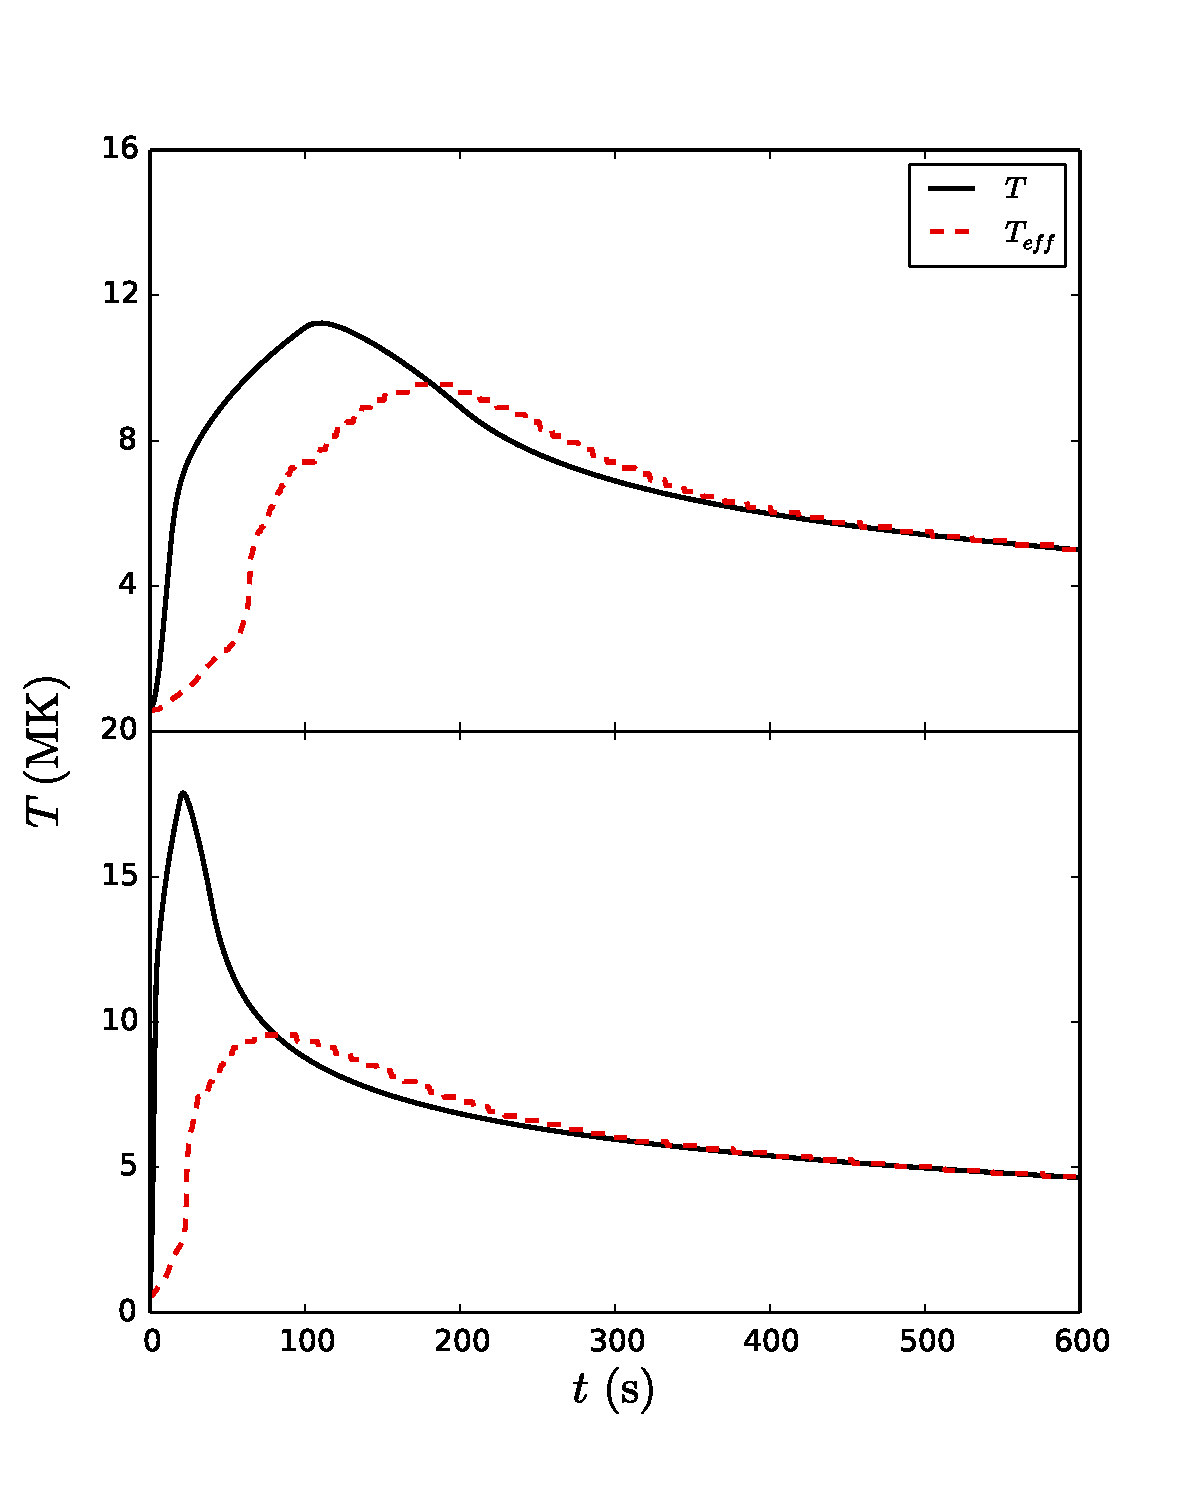
\includegraphics[width=\columnwidth]{figures/tt_eff_compare.pdf}
		\caption{The temperature (solid line) and effective temperature ($T_{eff}$: see text: dashed line) for two nanoflares. Both have a total energy input of 10 ergs cm$^{-3}$ s$^{-1}$. In the top (bottom) panel the nanoflare duration is 200 (40) s. The loop half-length is 40 Mm and only the first 600 s of the evolution are shown.}
		\label{fig:nei_ex}
	\end{figure}
	%
	\section{Results}
	\label{sec:results}
	%
	\par We now show a series of nanoflare simulations with our zero-dimensional hydrodynamic EBTEL model \citep{klimchuk_highly_2008, cargill_enthalpy-based_2012, cargill_enthalpy-based_2012-1, cargill_modelling_2015} and our modified two-fluid EBTEL model, first for single nanoflares and then in \citetalias{barnes_inference_2016-1} for distributions of nanoflares. 
	%
	\subsection{Single-fluid, Spitzer Conduction, Ionization Equilibrium}
	\label{subsec:sf_sc_ie_res}
	%
	\par In the first set of results we assume the plasma behaves as a single fluid, and ignore heat flux limiting and ionization non-equilibrium. \autoref{fig:vary_tau} shows $\mathrm{EM}(T)$ for a single nanoflare in a loop with $2L = 80$ Mm, and a heating function that takes the form of a triangular pulse and injects a total of 10 ergs cm$^{-3}$. These parameters correspond roughly to the bright AR core loops. We first vary the peak heating rate and pulse duration such that the total energy input is the same. Four cases are shown: pulses of 500, 200, 50 and 20 s duration which are the black dashed, solid, dashed-dotted and dotted lines respectively. The temperature and value of the peak emission measure are the same in all cases. (The red lines are discussed in \autoref{subsec:nei_res}).
	\begin{figure}
		\centering
		\caption{$\mathrm{EM}(T)$ for a nanoflare in an AR loop with $2L = 80$ Mm. The four curves correspond to different pulse durations: 500 s (dash-dot), 200 s (dash), 50 s (solid) and 20 s (dotted). The flux limiter is not applied. The red lines are calculated by binning $\mathrm{EM}$ using $T_{eff}$ (see \autoref{subsec:nei_res}).}
		\label{fig:vary_tau}
	\end{figure}
	%
	\par The values of $T_m$ and $\mathrm{EM}(T_m)$ are consistent with those found in the studies of core loops. Shorter pulses lead to higher initial temperatures, but the shape of the emission measure below $T_m$ is independent of the properties of the heating pulse, indicating that this part of the emission measure distribution cannot provide information about the actual nanoflare duration.  All cases show evidence of the heating phase, namely the bump on $\mathrm{EM}(T)$ at $\log{(T)} =$ 6.85, 7, 7.2 and 7.3, and is most obvious for the longer pulses. 
	\par Below these bumps the emission measure scales as $T^{-5}$  $T^{-5.5}$ to close to $T_m$ for all cases, again indicating that information of the heating process is lost. However, detection of such emission above $T_m$ would be evidence for nanoflare heating, though of undetermined duration.  For integration over the lifetime of unresolved structures lying transverse to the line of sight, one can write down an expression $\mathrm{EM}(T) \sim n^2\tau_{cool}(n, T)$ which simply states that what matters for determining $\mathrm{EM}(T)$ is how long the plasma spends at any given temperature \citep[e.g.][]{cargill_implications_1994,cargill_nanoflare_2004}. For an analytic solution for the cooling, one can formally define $\tau_{cool}(n, T) = (T/(dT/dt))$. In the absence of a formal solution, order of magnitude scalings can be used: the difference with analytic solutions being a numerical factor. To obtain an expression $\mathrm{EM}(T) ~ T^{-b}$, one needs to provide a relation between $T$ and $n$. For conductive cooling of the corona, one can write $\tau_{cool} \sim nL^2T^{-5/2}$, giving $\mathrm{EM} \sim n^3L^2T^{-5/2}$. In determining the relationship between $T$ and $n$, two limits are those of constant density and constant pressure. The former gives static conductive cooling \citep[e.g.][]{antiochos_influence_1976} and the latter evaporative cooling with constant thermal energy \citep[e.g.][]{antiochos_evaporative_1978}, which then lead to $b = 5/2$ and $11/2$ respectively. Our results are consistent with the latter.
	The three panels of \autoref{fig:vary_hdl} show the effect of varying the total nanoflare heating, the background density and the loop length. In all cases the pulse length is 200 s.
	%
	\begin{figure}
		\centering
		\caption{The effect of varying the magnitude of the heating (upper), the background density (middle) and the loop half-length (lower). The changes in each parameter are shown on each panel.}
		\label{fig:vary_hdl}
	\end{figure}
	%
	\par In all cases, the signature of nanoflare heating around and above 10 MK persists. When the heating amplitude increases, the value of $T_m$ increases above the values seen in AR cores, suggesting an upper limit on the nanoflare energy \citep[and hence on the time between nanoflares; see][]{cargill_active_2014}. It is important to note that changing the background density by an order of magnitude retains the hot component. This suggests that even in the intermediate frequency nanoflare regime there should be signatures above $T_m$.
	%
	\subsection{Heat Flux Limiter}
	\label{subsec:hf_res}
	%
	\autoref{fig:vary_fl} shows equivalent results to \autoref{fig:vary_tau}, but with a heat flux limiter included. Two values of $f$, $1/6$ (dashed line) and $1/30$ (dotted) are shown.
	\begin{figure}
		\centering
		\caption{$\mathrm{EM}(T)$ for a nanoflare in an AR loop with $2L = 80$ Mm with a flux limiter applied to the thermal conduction. The heating pulse lasts 200 s. The solid curve is as in \autoref{fig:vary_tau}, the dashed and dotted have the parameter $f = 1/6$ and $1/30$ respectively. The red curves are described in \autoref{subsec:nei_res}. The lower part of $\mathrm{EM}(T)$ is omitted: the profiles there for all cases are as in \autoref{fig:vary_tau}.}
		\label{fig:vary_fl}
	\end{figure}
	%
	\par As expected, inclusion of a limiter extends $\mathrm{EM}(T)$ to higher temperatures, however this is only notable above 10 MK. As the temperature falls to this value, evaporative upflows have increased the coronal density so that the Spitzer description is recovered. Above 10 MK flux limiting gradually becomes important, albeit with a small emission measure. For this case $\tau_{cool} \sim LT^{-1/2}$ so that the parameter $b$ lies between 1/2 and 5/2, depending on the assumption about $n$. For $f = 1/30$, $b = 5/2$ is found in \autoref{fig:vary_fl} \hl{Should we show this explicitly?}. Since the free streaming limit slows conduction cooling relative to that given by Spitzer, the plasma will spend more time at any given temperature, leading to smaller values of $b$. Similar conclusions hold for other conduction models \citep[e.g. the non-local model discussed in the coronal context by][]{karpen_nonlocal_1987,west_lifetime_2008} since they all inhibit conduction. While limiting of conduction is often regarded as an important process in coronal cooling, these results suggest that for nanoflare heating it may not be that important.
	%
	\subsection{Multi-fluid Modeling}
	\label{subsec:two_fluid_res}
	%
	\hl{Two-fluid results go here.}
	%
	\subsection{Ionization Non-equilibrium}
	\label{subsec:nei_res}
	%
	\par Results for ionization non-equilibrium are shown in red on \autoref{fig:vary_tau},\autoref{fig:vary_hdl},\autoref{fig:vary_fl}. With the exception of the case of the extreme flux limiter value of $f = 1/30$, the effect is to truncate the $\mathrm{EM}(T)$ profile to around or below 10 MK. The bump on the distribution characteristic of the heating phase is also relocated to lower temperatures. In \autoref{fig:vary_tau} it is also shown that any pulse length $< 200$ s leads to very similar $\mathrm{EM}-T_{eff}$ profiles.
	%
	\par There are two effects that lead to temperatures below 10 MK. The first is that for long pulses $> 200$ s, the heating is in direct competition with thermal conduction, which thus limits the temperature to these values. Secondly, the short pulses reach the higher temperatures too quickly for the ionization state of the plasma to keep up, and this only happens at or below 10 MK. Thus it seems as if the temperature range $T_m$ up to 10 MK is the optimal one for searching for this hot component as well as direct signatures of the heating. It is though difficult to ``map'' what would be seen in such a state of ionization non-equilibrium back to the real system.
	%
	\section{Discussion}
	\label{sec:discussion}
	%
	\par In this paper we have looked at the hot plasma component that arises from a single nanoflare. It is shown that this component is ubiquitous and has a distribution of emission measure as a function of temperature consistent with conductive cooling for either Spitzer of free-streaming conduction models. There is a characteristic ``bump'' on the emission measure at or above 10 MK that is a direct manifestation of the heating process. While both these results suggest quantitative ways of measuring this plasma in the future, there is an important caveat. That is the lack of ionization equilibrium leads to a failure to be actually able to observe this hot plasma in most cases.
	%
	\par From the single nanoflare results for a single fluid, it appears that it is not possible to say anything about the plasma in excess of 10 MK. If the electrons are heated, this plasma exists, with electron temperature in excess of 10 MK, but nothing can be said about it. It is effectively a ``dark'' hot plasma. The case of proton heating is even more complicated. On the other hand, the bump on $\mathrm{EM}(T)$ associated with the heating does seem to be shifted down in temperature.
	%
	\par A full discussion of where this leads for present and future measurements will be deferred to paper 2 where we discuss results for nanoflare trains, including the important ``intermediate frequency'' nanoflare case. But one can conclude (i) present day observations do not seem capable of making quantitative statements about the ``hot'' component, though they are highly suggestive of its existence and (ii) future measurements should be concentrated in the temperature regime $10^{6.6}$ – $10^7$ K rather than at higher temperatures. The MaGIXS instrument, due to fly in 2017, is well positioned to do this. Finally, the rocket results of \citet{caspi_new_2015} pose a problem in that if only quiescent coronal plasma were being observed, it is difficult to understand how an emission measure distribution characteristic of Spitzer conduction can arise. It seems possible that a microflare or small flare occurred during the observations.
	%
	\appendix
	\section{}
	\label{appendix}
	%
	\par\hl{Derivation of two-fluid equations goes here.}
	%
	%
	%Bibliography
	\bibliography{astrophys-abbrev.bib,references.bib}
	\bibliographystyle{apj}
	\clearpage
\end{document}